\documentclass[12pt,a4paper]{article}

% --- Paquetes ---
\usepackage[utf8]{inputenc}
\usepackage[spanish]{babel}
\usepackage{amsmath, amssymb, amsfonts}
\usepackage{graphicx}
\usepackage{geometry}
\usepackage{booktabs}
\usepackage{hyperref}
\usepackage{subcaption}
\usepackage{float}

% --- Configuración de Página ---
\geometry{left=2.5cm,right=2.5cm,top=2.5cm,bottom=2.5cm}

\begin{document}
\setlength{\parskip}{1em}    
\setlength{\parindent}{2em}

\begin{titlepage}
    \centering
    {\bfseries\LARGE UNIVERSIDAD NACIONAL DE INGENIERÍA \par}
    \vspace{0.5cm}
    {\bfseries\Large FACULTAD DE CIENCIAS \par}
    {\bfseries\large Escuela Profesional de Ciencia de la Computación\par}
    \begin{figure}[H]
        \centering
        
\includegraphics[width=8cm]{img/uni_logo.png}
    \end{figure}
    {\scshape TAREA ACADÉMICA:   \par}
    {\bfseries Predicción de Heladas Meteorológicas en el Perú mediante un Pipeline de Aprendizaje Automático Robusto a Anomalías: Imputación por Mediana, Escalamiento Robusto, PCA y Random Forest Optimizado \par}
    {\Large\bfseries  \par}
    \vfill
    {\scshape ELABORADO POR: \par}
    {\bfseries Meiser Brayan Gamboa Cuello \par}
    {\bfseries Lino Alejandro Taipe Mendivil \par}
    {\Large\bfseries  \par}
    \vfill
    {\Large (Lima - Perú) \par}
    {\Large 2026 \par}
\end{titlepage}
    
% --- Datos del Informe ---
\title{\textbf{Predicción de Heladas Meteorológicas en el Perú mediante un Pipeline de Aprendizaje Automático Robusto a Anomalías: Imputación por Mediana, Escalamiento Robusto, PCA y Random Forest Optimizado}}
\author{
Meiser Brayan Gamboa cuello \\ 
\small Universidad Nacional de Ingeniería \\
\small meiser.gamboa.c@uni.pe
\and
Lino Alejandro Taipe Mendivil \\ 
\small Universidad Nacional de Ingeniería \\
\small c@uni.pe
}
\date{
\small
Curso: Minería de Datos (CC442) --- Ciclo 2026-I\\
Profesor: Dr. Marcos Antonio Alania Vicente\\[0.5em]
\today
}
\maketitle

\begin{abstract}
Las heladas meteorológicas son uno de los eventos climáticos extremos de mayor
impacto sobre la agricultura altoandina del Perú, generando pérdidas severas en
cultivos y ganado. Su predicción temprana constituye un problema de
clasificación binaria fuertemente desbalanceado, en el que los clasificadores
convencionales favorecen la clase mayoritaria. A diferencia de trabajos previos
que abordan este desbalance mediante sobremuestreo sintético (SMOTE) y suelen
omitir la corrección de anomalías de instrumentación, este trabajo propone un
pipeline de minería de datos que combina corrección explícita de errores de
sensor, ponderación balanceada de clases y optimización orientada a la clase
minoritaria. Sobre 1\,672\,827 observaciones meteorológicas horarias de
estaciones peruanas (18 variables), se identificó y corrigió un código de error
de sensor (\texttt{-999}) no documentado, se definió la variable objetivo
mediante el umbral físico de $0^{\circ}\text{C}$ y se eliminó el predictor
definitorio para evitar fuga de información. El preprocesamiento aplicó
imputación por mediana y \texttt{RobustScaler}, seguido de PCA que redujo el
espacio de 15 a 5 componentes reteniendo el 95\% de la varianza. Se entrenó un
\emph{Random Forest Classifier} balanceado, optimizado mediante
\texttt{GridSearchCV} (3-fold, F1-Score Macro). El modelo alcanzó un
\emph{Recall} de 92.34\% y un \emph{F1-Score} macro de validación de 0.8330 en
la detección de heladas, con un índice Kappa de Cohen de 0.6710, evidenciando
concordancia sustancial. Los resultados validan el sistema como herramienta de
alerta temprana de alta sensibilidad para la prevención de desastres
agrometeorológicos.

\vspace{0.5cm}
\noindent \textbf{Palabras clave:} 
Agriculture, data mining, meteorology, predictive models, principal component
analysis, random forests.
\end{abstract}
\section{Introduction}

Las heladas meteorológicas, definidas como el descenso de la
temperatura del aire por debajo de $0^{\circ}\text{C}$, constituyen uno de los
fenómenos climáticos extremos de mayor recurrencia en las zonas altoandinas del
Perú. En un país donde amplios sectores de la población rural dependen de una
agricultura y ganadería de subsistencia altamente sensibles a la variabilidad
térmica nocturna, estos eventos representan una amenaza estructural para la
seguridad alimentaria y la estabilidad económica de las comunidades más
vulnerables. La creciente irregularidad de los patrones climáticos ha
intensificado la frecuencia y severidad de estos episodios, situando su
predicción anticipada como un problema de relevancia nacional.

Desde una perspectiva socioeconómica, la ocurrencia de una helada puede destruir
en cuestión de horas la totalidad de un cultivo sensible, provocando pérdidas
directas para el productor y presionando las cadenas de abastecimiento
regionales. La capacidad de anticipar estos eventos con antelación suficiente
permite activar medidas de mitigación en campo, reduciendo el impacto económico
y protegiendo los medios de vida de las poblaciones afectadas. Técnicamente, sin
embargo, los modelos numéricos de predicción meteorológica tradicionales suelen
carecer de la resolución espacial necesaria para capturar los microclimas
locales que determinan la ocurrencia de heladas a escala puntual. En este
contexto, los métodos de aprendizaje automático supervisado, entrenados
directamente sobre registros históricos de estaciones meteorológicas, han
emergido como una alternativa computacionalmente eficiente y de bajo costo para
la predicción de estos eventos a nivel local
\cite{diedrichs2018,talsma2023,rozante2023,perez2025}.

No obstante, la aplicación efectiva de estas técnicas sobre datos meteorológicos
reales impone desafíos que trascienden la simple selección de un algoritmo. En
términos de minería de datos, la predicción de heladas se formula como un
problema de \emph{clasificación binaria supervisada fuertemente desbalanceado},
en el que la clase de interés (ocurrencia de helada) es estadísticamente
minoritaria frente a las condiciones climáticas normales. Este desbalance sesga
a los clasificadores convencionales hacia la clase mayoritaria, tornando
inadecuadas métricas como la exactitud y exigiendo estrategias explícitas de
mitigación \cite{azhar2023,wang2021}. A este desafío se suman tres
complicaciones inherentes al dominio: (i) la presencia de códigos de error de
instrumentación no documentados que contaminan la topología estadística de los
datos crudos; (ii) el riesgo de fuga de información (\emph{data leakage}) al
derivar la variable objetivo a partir de una medición física que, de conservarse
entre los predictores, induciría una regla determinista trivial; y (iii) la alta
multicolinealidad entre variables climáticas interdependientes, que introduce
redundancia y degrada la convergencia del modelado. El presente trabajo aborda
integralmente estos cuatro aspectos mediante un pipeline reproducible diseñado
específicamente para el contexto meteorológico peruano.

Las principales contribuciones de este trabajo son:
\begin{enumerate}
\item Se identifica y corrige de forma sistemática un código de error de sensor
(\texttt{-999}) no documentado en el conjunto de datos crudo, mediante un
diagnóstico exploratorio comparativo de las funciones de densidad antes y después
de la corrección, recuperando la topología estadística real de las variables.
\item Se diseña una variable objetivo físicamente fundamentada
(\emph{Target\_Helada}) a partir del umbral termodinámico de $0^{\circ}\text{C}$,
eliminando explícitamente el predictor definitorio del espacio de características
para prevenir la fuga de información por predicción tautológica.
\item Se construye un pipeline de preprocesamiento robusto a valores atípicos
físicamente válidos, combinando imputación por mediana y \texttt{RobustScaler},
justificado matemáticamente frente a la estandarización clásica y a la
eliminación de \emph{outliers}, seguido de una reducción de dimensionalidad
mediante Análisis de Componentes Principales (PCA) que retiene el 95\% de la
varianza empírica.
\item Se optimiza un \emph{Random Forest Classifier} con ponderación balanceada
de clases mediante \texttt{GridSearchCV}, empleando el F1-Score Macro como función
objetivo para penalizar directamente los falsos negativos críticos, en lugar de
recurrir al sobremuestreo sintético empleado por trabajos previos.
\item Se realiza una evaluación integral del modelo mediante métricas robustas al
desbalance de clases (curva ROC-AUC, curva Precision-Recall e índice Kappa de
Cohen), acompañada de un análisis de la capacidad discriminante de los
componentes principales.
\end{enumerate}

El resto de este artículo está organizado de la siguiente manera. La
Sección~\ref{sec:relwork} presenta los trabajos relacionados y una comparación
sistemática con el enfoque propuesto. La Sección~\ref{sec:dataset} describe el
conjunto de datos y el análisis exploratorio, incluyendo la detección de
anomalías. La Sección~\ref{sec:preprocessing} detalla el preprocesamiento
matemático de los datos. La Sección~\ref{sec:methodology} expone la metodología
propuesta, sus algoritmos y la estrategia de optimización. La
Sección~\ref{sec:implementation} describe la implementación de software y las
consideraciones de reproducibilidad. La Sección~\ref{sec:results} presenta los
resultados experimentales. La Sección~\ref{sec:discussion} interpreta los hallazgos, sus
fortalezas y limitaciones. Finalmente, la Sección~\ref{sec:conclusions} presenta
las conclusiones y el trabajo futuro.
\section{Trabajos Relacionados}\label{sec:relwork}
 
La predicción de heladas mediante aprendizaje automático ha sido abordada en múltiples contextos agroclimáticos. Diedrichs et al. \cite{diedrichs2018} desarrollaron un sistema de soporte a la decisión basado en Random Forest y regresión logística sobre datos de estaciones meteorológicas de la provincia de Mendoza (Argentina), aplicando SMOTE para mitigar el desbalance de clases. Talsma et al. \cite{talsma2023} compararon redes neuronales profundas, redes convolucionales y Random Forest para la predicción de heladas a múltiples horizontes temporales (6--48 h) en Nuevo México (EE.\,UU.), reportando errores de predicción de temperatura mínima entre 1.53 y 1.72\,$^{\circ}$C. Rozante et al. \cite{rozante2023} emplearon perceptrones multicapa (MLP) con optimizadores ADAM y SGD para mejorar las predicciones del modelo numérico Eta en el sur de Brasil. Más recientemente, Pérez Tárraga et al. \cite{perez2025} compararon un conjunto amplio de algoritmos de clasificación, incluyendo Random Forest, sobre datos de la Agencia Estatal de Meteorología de España (AEMET), aplicando igualmente SMOTE para el desbalance de clases y concluyendo que Random Forest ofrece el mejor desempeño para horizontes cortos ($\leq$24\,h).
 
En el ámbito específico del manejo de clases desbalanceadas, Azhar et al. \cite{azhar2023} realizaron una revisión comparativa exhaustiva de variantes de SMOTE frente a distintas complejidades de datos (ruido, solapamiento de clases, subconjuntos pequeños). Wang et al. \cite{wang2021} presentaron una revisión sistemática de métodos de clasificación sobre conjuntos de datos desbalanceados, cubriendo tanto técnicas a nivel de datos como a nivel de algoritmo. Zhao \cite{zhao2024} propuso una variante de SMOTE basada en grafos de vecindad natural con núcleos de subgrafos para mejorar la calidad de las muestras sintéticas generadas.
 
Respecto a la reducción de dimensionalidad en dominios meteorológicos, Galván et al. \cite{galvan2022} compararon PCA frente a métodos de reducción supervisada (LPP, LOL, SNMF) para el pronóstico de radiación solar a partir de rejillas meteorológicas de alta dimensionalidad, señalando las limitaciones del carácter lineal y no supervisado de PCA. En cuanto a la optimización de hiperparámetros, Bujang et al. \cite{bujang2021} evaluaron \texttt{GridSearchCV} y métodos alternativos (búsqueda aleatoria, algoritmos genéticos, Bayesianos) para la calibración de modelos de clasificación de Random Forest, mientras que Chen et al. \cite{chen2024soil} aplicaron Random Forest a la predicción estacional de contenido hídrico del suelo agrícola a partir de datos de precipitación, evidenciando la versatilidad del algoritmo en tareas de agrometeorología de precisión.
 
La Tabla \ref{tab:relwork} resume los trabajos más relevantes revisados, publicados en los últimos cinco años en las bases IEEE Xplore, Springer, ACM y ScienceDirect, en comparación con el enfoque propuesto en este artículo.
 
\begin{table}[H]
\centering
\caption{Comparación de trabajos relacionados publicados en los últimos cinco años}
\label{tab:relwork}

\resizebox{\textwidth}{!}{%
\begin{tabular}{p{2.6cm}p{1.4cm}p{2.6cm}p{3.3cm}p{3.4cm}p{2.5cm}}
\toprule
\textbf{Referencia} & \textbf{Año} & \textbf{Fuente} & \textbf{Dominio} & \textbf{Método principal} & \textbf{Manejo de desbalance} \\
\midrule
Rozante et al. \cite{rozante2023} & 2023 & ScienceDirect & Predicción de heladas (Brasil) & MLP (ADAM/SGD) & No reportado \\
Pérez Tárraga et al. \cite{perez2025} & 2025 & Springer (Earth Sci. Informatics) & Predicción de heladas (España) & Comparación de clasificadores (incl. RF) & SMOTE \\
Azhar et al. \cite{azhar2023} & 2023 & IEEE TKDE & Datos desbalanceados (general) & Revisión comparativa de variantes SMOTE & SMOTE (múltiples variantes) \\
Wang et al. \cite{wang2021} & 2021 & IEEE Access & Clasificación desbalanceada (general) & Revisión sistemática & Nivel de datos y de algoritmo \\
Zhao \cite{zhao2024} & 2024 & Springer (J. Supercomputing) & Datos desbalanceados (general) & SMOTE sobre grafo de vecindad natural & SMOTE mejorado \\
Bujang et al. \cite{bujang2021} & 2021 & IEEE Access & Predicción académica & Random Forest + optimización de hiperparámetros & \texttt{class\_weight} / búsqueda en grilla \\
Galván et al. \cite{galvan2022} & 2022 & Springer (Applied Intelligence) & Pronóstico de radiación solar & PCA + métodos supervisados de reducción & No aplica \\
Chen et al. \cite{chen2024soil} & 2024 & ScienceDirect & Contenido hídrico del suelo & Random Forest & No aplica \\
\midrule
\textbf{Propuesta (este trabajo)} & 2026 & --- & \textbf{Predicción de heladas (Perú)} & \textbf{RobustScaler + PCA + RF con \texttt{class\_weight = 'balanced'} y GridSearchCV} & \textbf{Ponderación balanceada de clases + optimización sobre F1-Macro} \\
\bottomrule
\end{tabular}%
}

\end{table}
 
A diferencia de los trabajos previos, que en su mayoría emplean SMOTE como técnica principal de rebalanceo, el presente trabajo opta por la ponderación de clases (\texttt{class\_weight='balanced'}) combinada con optimización directa sobre F1-Score Macro, evitando la generación de muestras sintéticas en un espacio de alta dimensionalidad ya afectado por anomalías de sensor, y complementa el preprocesamiento con una corrección explícita de códigos de error de instrumentación no reportada en los estudios comparados.
 
\section{Descripción del Dataset y Análisis Exploratorio}\label{sec:dataset}

\subsection{Origen y dominio de aplicación}
El conjunto de datos empleado es de acceso \emph{público} y proviene del
repositorio Kaggle bajo el identificador
\texttt{abadpomamaquera/meteorological-data-for-frost-prediction-in-peru}. La
ingesta se realizó de forma programática mediante la librería \texttt{kagglehub}
con el adaptador \texttt{KaggleDatasetAdapter.PANDAS}. El dominio de aplicación
corresponde a la \emph{meteorología agrícola} de las regiones altoandinas del
Perú, y la unidad de observación es un registro meteorológico horario asociado a
estaciones de medición. Según la documentación oficial del repositorio, el
dataset integra variables atmosféricas y geográficas comúnmente asociadas a la
formación de heladas, seleccionadas por su relevancia en estudios agroclimáticos
y ambientales.

El repositorio ofrece dos versiones: \texttt{DATASET.csv}, descrito como el
conjunto completo tras un preprocesamiento inicial, y
\texttt{DATASET\_FILTRADO.csv}, la versión filtrada empleada por el autor
original para entrenar un clasificador XGBoost. El presente trabajo utiliza
deliberadamente la versión \texttt{DATASET.csv} con un clasificador Random Forest,
constituyendo un pipeline de preprocesamiento y modelado independiente del
propuesto por el autor del repositorio, lo que permite un contraste metodológico.

\subsection{Tamaño, instancias y características}
El archivo \texttt{DATASET.csv} ocupa $301.77$\,MB en disco según la
documentación oficial del repositorio. La matriz cargada contiene
$N = 1\,672\,827$ instancias y $D = 18$ características, con una huella real en
memoria de $229.7$\,MB según \texttt{df.info()}. En cuanto a los tipos de dato,
16 variables son de punto flotante (\texttt{float64}) y 2 son enteras
(\texttt{int64}), correspondientes a las variables temporales \texttt{año} y
\texttt{dia}.

\subsection{Observación sobre la calidad de los datos}
Aunque la documentación del repositorio describe \texttt{DATASET.csv} como un
conjunto ``limpio y estandarizado'' del que se habrían removido los registros
faltantes e inconsistentes, el análisis exploratorio realizado en este trabajo
detectó que dicha versión \emph{conserva} el código de error de sensor
\texttt{-999} sin corregir (Fig.~\ref{fig:eda_raw}). Adicionalmente, se identificó
una discrepancia entre la documentación y el contenido efectivo del archivo: la
ficha oficial menciona un ``balance de radiación'' entre las variables, pero el
análisis de las 18 columnas no identifica ninguna variable de radiación; las
columnas efectivamente presentes son las 18 listadas en la Tabla~\ref{tab:dict},
incluyendo coordenadas geográficas (\texttt{latitud}, \texttt{longitud}) y
\texttt{altitud}. Estas observaciones justifican la etapa de corrección de
anomalías descrita en la Sección~\ref{sec:preprocessing} y refuerzan la necesidad
de un diagnóstico independiente de la calidad de los datos, incluso cuando la
fuente los declara preprocesados.

\subsection{Diccionario de variables}
La Tabla~\ref{tab:dict} presenta el diccionario de variables con sus rangos
empíricos reales, obtenidos mediante \texttt{df.describe()}. Se observa que 13 de
las 16 variables continuas presentan un valor mínimo de \texttt{-999},
correspondiente al código de error de sensor; en contraste, las variables
temporales (\texttt{año}, \texttt{dia}) y geográficas (\texttt{latitud},
\texttt{longitud}, \texttt{altitud}) presentan rangos físicamente válidos, lo que
valida la aplicación selectiva del filtro de corrección. Los rangos de
\texttt{latitud} $[-18.01, -8.19]$ y \texttt{longitud} $[-78.04, -69.06]$
confirman geográficamente la procedencia peruana de las estaciones.

\begin{table}[H]
\centering
\caption{Diccionario de variables con rangos empíricos ($N=1\,672\,827$)}
\label{tab:dict}
\scriptsize
\renewcommand{\arraystretch}{1.15}
\begin{tabular}{p{1.9cm}p{0.7cm}p{1.9cm}p{2.2cm}}
\toprule
\textbf{Variable} & \textbf{Tipo} & \textbf{Rango [min, max]} & \textbf{Descripción física} \\
\midrule
\texttt{año} & entera & [2000, 2025] & Año del registro \\
\texttt{dia} & entera & [1, 366] & Día juliano del registro \\
\texttt{temp\_2m} & continua & [-999, 30.21] & Temperatura del aire a 2\,m ($^\circ$C) \\
\texttt{punto\_rocio\_2m} & continua & [-999, 20.84] & Punto de rocío a 2\,m ($^\circ$C) \\
\texttt{temp\_max\_2m} & continua & [-999, 36.77] & Temperatura máxima a 2\,m ($^\circ$C) \\
\texttt{temp\_min\_2m} & continua & [-999, 25.03] & Temperatura mínima a 2\,m; base de la etiqueta \\
\texttt{humedad\_rel\_2m} & continua & [-999, 99.74] & Humedad relativa a 2\,m (\%) \\
\texttt{viento\_2m} & continua & [-999, 7.47] & Velocidad del viento a 2\,m (m/s) \\
\texttt{viento\_max\_2m} & continua & [-999, 11.61] & Ráfaga máxima a 2\,m (m/s) \\
\texttt{viento\_min\_2m} & continua & [-999, 5.57] & Viento mínimo a 2\,m (m/s) \\
\texttt{viento\_10m} & continua & [-999, 10.49] & Velocidad del viento a 10\,m (m/s) \\
\texttt{viento\_max\_10m} & continua & [-999, 15.16] & Ráfaga máxima a 10\,m (m/s) \\
\texttt{viento\_min\_10m} & continua & [-999, 6.98] & Viento mínimo a 10\,m (m/s) \\
\texttt{humedad\_suelo} & continua & [-999, 0.98] & Humedad volumétrica del suelo \\
\texttt{precipitacion} & continua & [-999, 470.24] & Precipitación acumulada (mm) \\
\texttt{latitud} & continua & [-18.01, -8.19] & Latitud de la estación (grados) \\
\texttt{longitud} & continua & [-78.04, -69.06] & Longitud de la estación (grados) \\
\texttt{altitud} & continua & [1079.2, 4691.4] & Altitud de la estación (m.s.n.m.) \\
\midrule
\texttt{Target\_Helada} & binaria & \{0, 1\} & Etiqueta derivada: $1$ si $\texttt{temp\_min\_2m}\le 0^\circ$C \\
\bottomrule
\end{tabular}
\end{table}

\subsection{Distribuciones de las variables densas}
El análisis exploratorio inicial sobre los datos crudos reveló una anomalía
crítica de calidad: prácticamente todas las variables numéricas presentaban una
extensión de su soporte hacia valores físicamente imposibles, cercanos a
$-1000$, que comprimía la distribución real en una línea recta indistinguible
(Fig.~\ref{fig:eda_raw}). Esto evidenció que los sensores codificaron los fallos
de lectura mediante el valor de relleno \texttt{-999}. Tras la corrección
(Sección~\ref{sec:preprocessing}), las funciones de densidad recuperan su
topología termodinámica real (Fig.~\ref{fig:eda_clean}).

\begin{figure}[H]
\centering
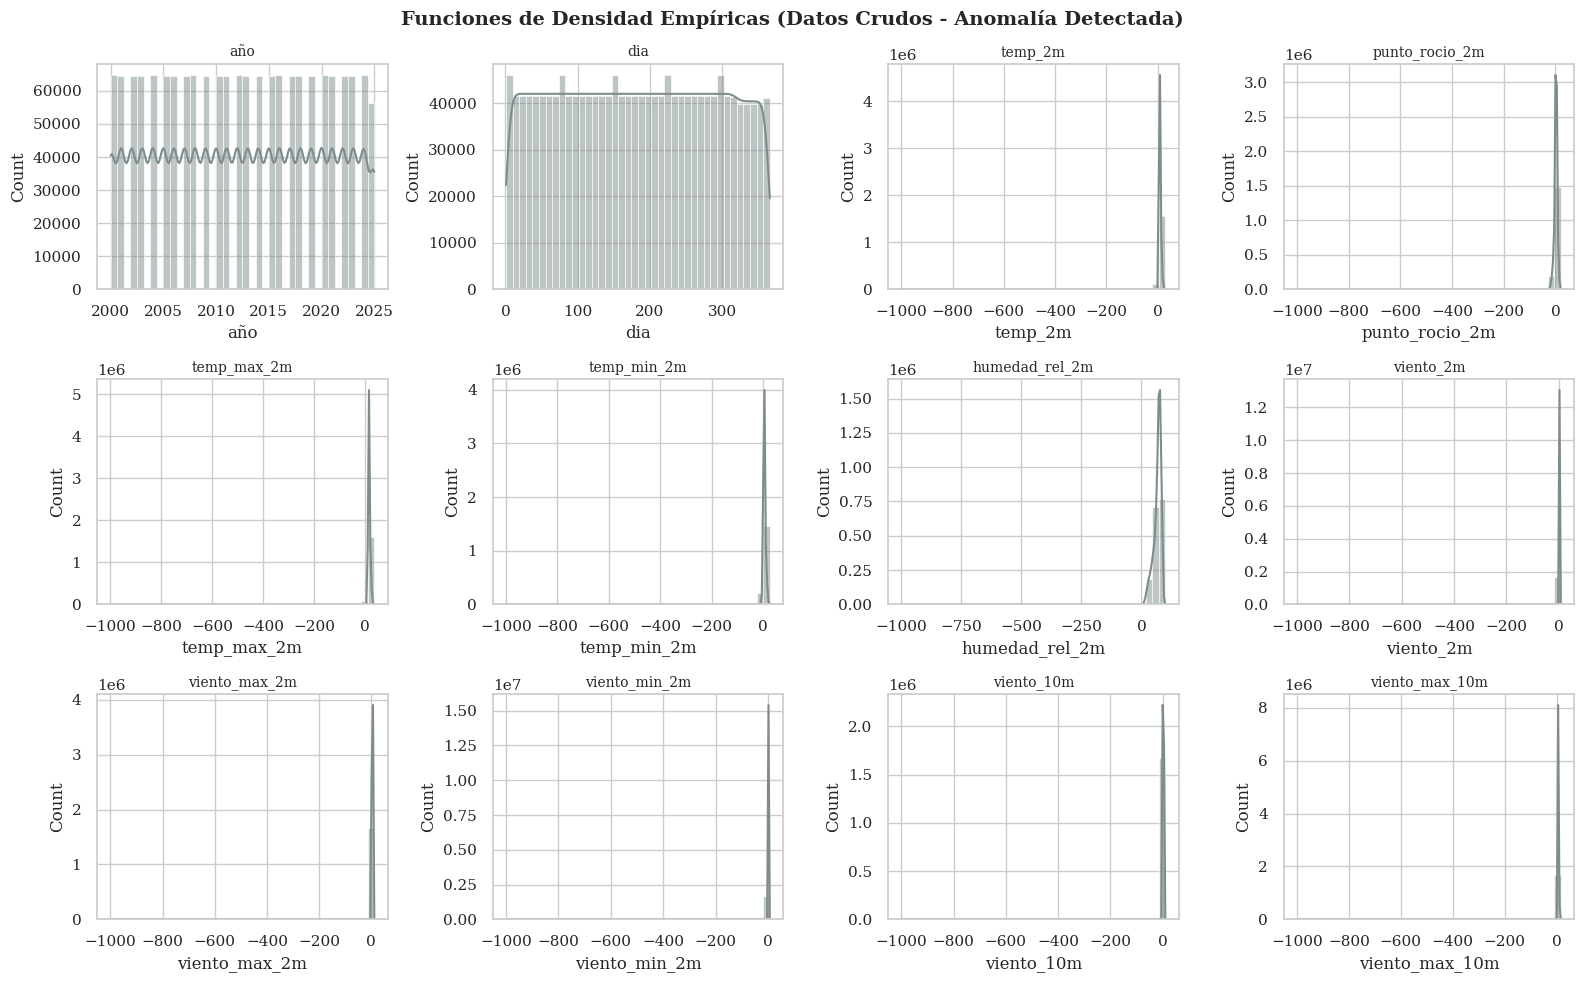
\includegraphics[width=1.00\textwidth]{img/cell4_out0.png}
\caption{Funciones de densidad empíricas sobre los datos crudos. La anomalía de
codificación de error (\texttt{-999}) colapsa las distribuciones reales.}
\label{fig:eda_raw}
\end{figure}

\begin{figure}[H]
\centering
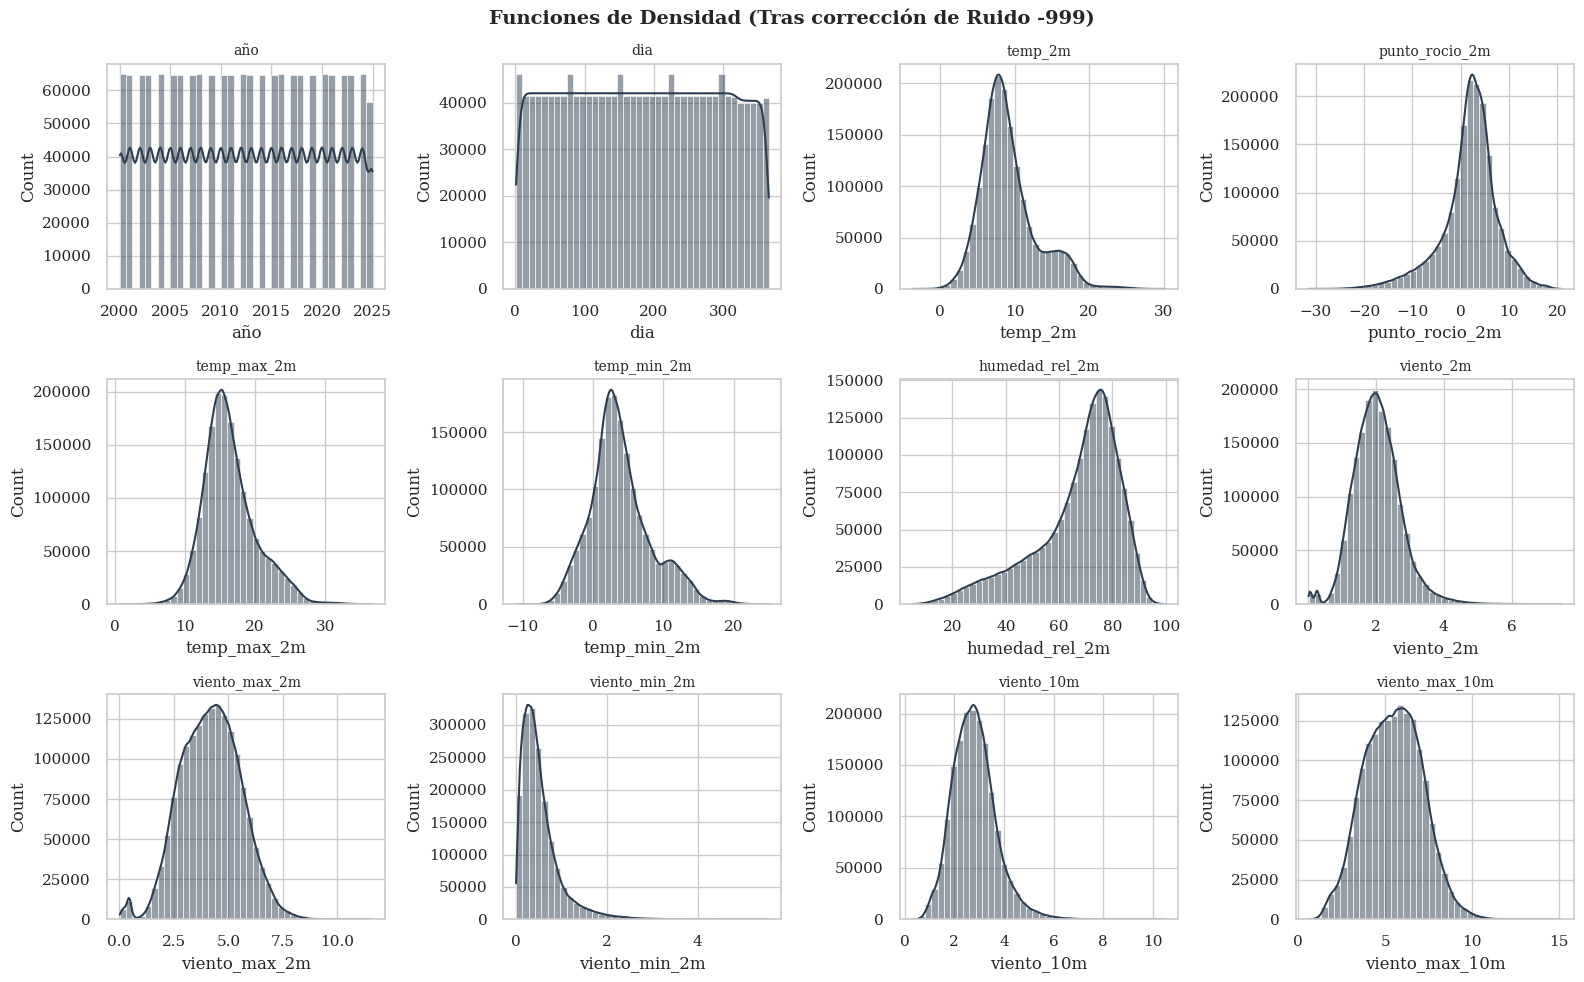
\includegraphics[width=1.00\textwidth]{img/cell6_out1.png}
\caption{Funciones de densidad empíricas tras la corrección del código de error
\texttt{-999}, mostrando la topología real de las variables meteorológicas.}
\label{fig:eda_clean}
\end{figure}

\subsection{Valores faltantes}
Un aspecto metodológicamente relevante es que el archivo original no contiene
valores nulos explícitos: la inspección estructural (\texttt{df.info()}) reporta
$1\,672\,827$ registros no nulos en las 18 columnas. Los datos faltantes se
encontraban \emph{enmascarados} bajo el código de error \texttt{-999}, y solo
emergen como nulos tras aplicar el filtro de corrección descrito en la
Sección~\ref{sec:preprocessing}. Una vez desenmascarados, la verdadera tasa de
datos faltantes resulta baja y homogénea: exactamente 531 registros por variable
numérica afectada, equivalentes al $0.031743\%$ del total
(Tabla~\ref{tab:missing}). Esta uniformidad sugiere un origen común de los fallos
de sensor, probablemente ventanas de mantenimiento o cortes simultáneos de
adquisición. La detección de este enmascaramiento constituye precisamente la
justificación de la etapa de corrección de anomalías, dado que un diagnóstico
superficial basado únicamente en \texttt{df.info()} habría concluido erróneamente
que el conjunto estaba libre de datos faltantes.

\begin{table}[H]
\centering
\caption{Tasa de valores faltantes tras desenmascarar el código de error}
\label{tab:missing}
\footnotesize
\begin{tabular}{lcc}
\toprule
\textbf{Variables afectadas} & \textbf{Faltantes} & \textbf{Porcentaje} \\
\midrule
13 variables numéricas & 531 c/u & $0.031743\%$ \\
\bottomrule
\end{tabular}
\end{table}

\subsection{Desbalance severo de clases}
El análisis de la variable objetivo confirmó un desbalance de clases agudo, un
problema crítico para el modelado posterior (Tabla~\ref{tab:imbalance}). La clase
de interés (ocurrencia de helada) representa apenas el $16.24\%$ de las
observaciones, lo que justifica el uso de ponderación balanceada de clases y de
métricas robustas al desbalance en lugar de la exactitud.

\begin{table}[H]
\centering
\caption{Distribución de la variable objetivo \emph{Target\_Helada}}
\label{tab:imbalance}
\footnotesize
\begin{tabular}{lcc}
\toprule
\textbf{Clase} & \textbf{Instancias} & \textbf{Porcentaje} \\
\midrule
0 (Normal) & 1\,401\,118 & $83.757496\%$ \\
1 (Helada) & 271\,709 & $16.242504\%$ \\
\midrule
\textbf{Total} & \textbf{1\,672\,827} & $100\%$ \\
\bottomrule
\end{tabular}
\end{table}

\subsection{Correlación lineal (Pearson)}
Se calculó la matriz de correlación lineal de Pearson sobre una submuestra de
$\min(N, 20\,000)$ registros completos, con semilla fija ($\text{SEED}=42$),
visualizada mediante un mapa de calor con máscara triangular superior
(Fig.~\ref{fig:corr}). Las cinco variables con mayor correlación lineal absoluta
respecto a la helada fueron \texttt{punto\_rocio\_2m} ($r=0.5581$),
\texttt{temp\_2m} ($r=0.4867$), \texttt{altitud} ($r=0.3779$),
\texttt{humedad\_rel\_2m} ($r=0.3007$) y \texttt{temp\_max\_2m} ($r=0.2856$). El
mapa evidencia además alta multicolinealidad entre grupos de sensores
relacionados (variantes de viento y de temperatura), lo que motiva la reducción
de dimensionalidad mediante PCA.

\begin{figure}[H]
\centering
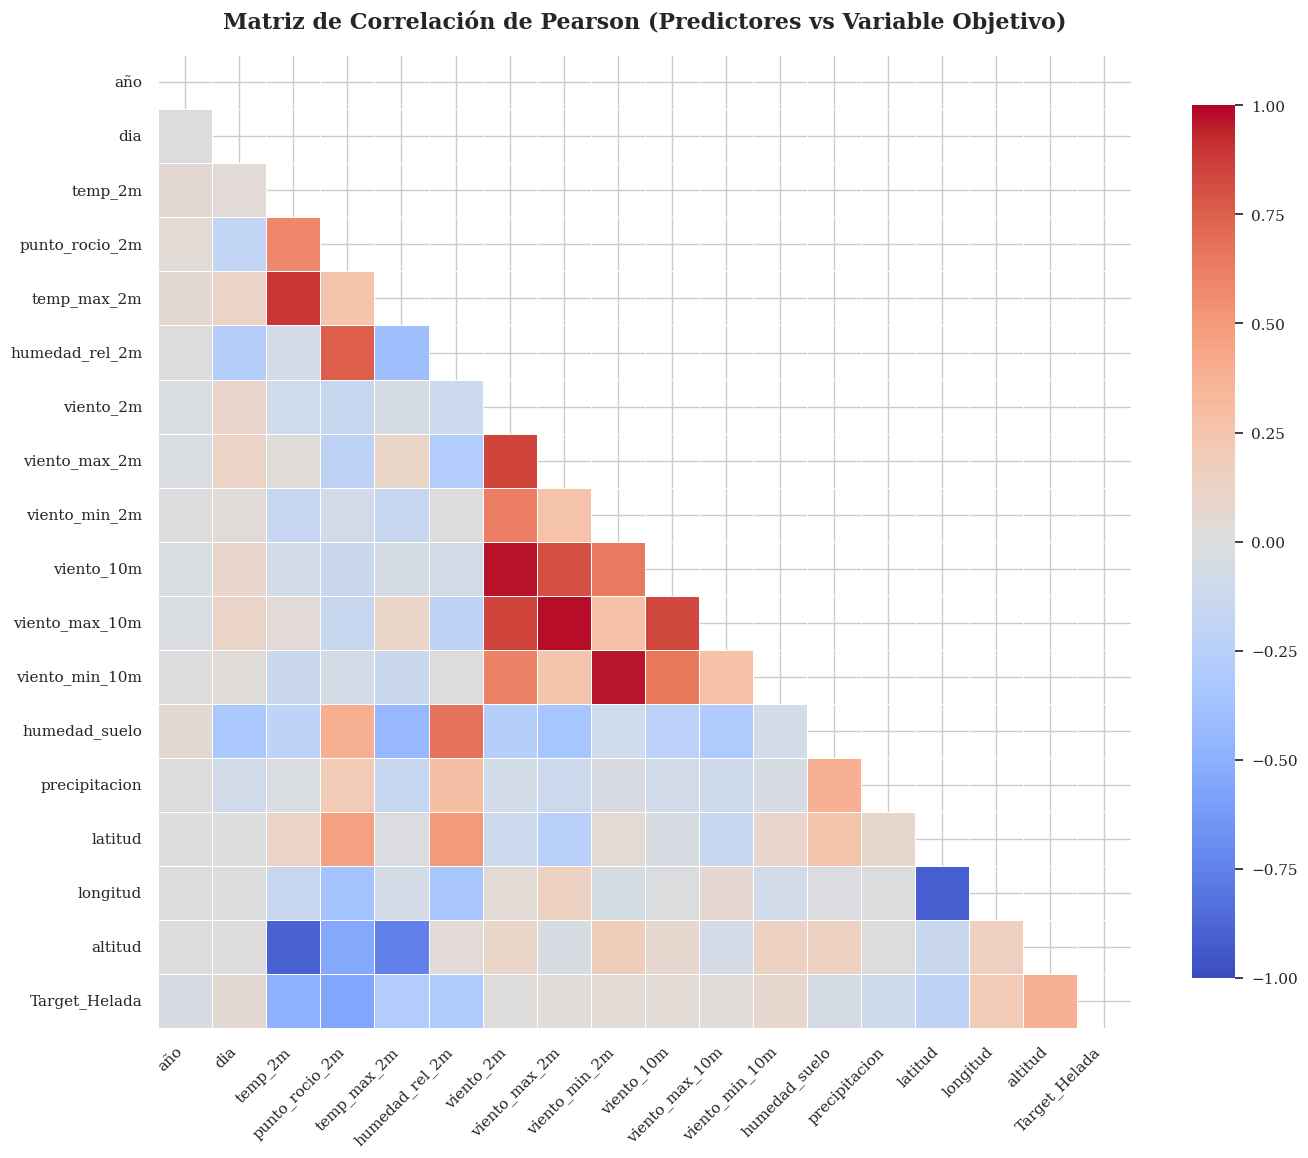
\includegraphics[width=1.00\textwidth]{img/cell8_out2.png}
\caption{Matriz de correlación lineal de Pearson entre predictores y la variable
objetivo \emph{Target\_Helada}.}
\label{fig:corr}
\end{figure}

\subsection{Valores atípicos univariados legítimos}
Más allá del artefacto \texttt{-999}, el análisis de los estadísticos descriptivos
revela un valor atípico físicamente legítimo en la variable
\texttt{precipitacion}: su máximo alcanza $470.24$\,mm frente a un tercer cuartil
de apenas $0.87$\,mm y una mediana de $0.04$\,mm (Tabla~\ref{tab:dict}). Este
valor no constituye un error de sensor sino un evento de precipitación extrema
real. Coherentemente con el tratamiento adoptado para las heladas, tales extremos
se preservan como señal y se protegen mediante el escalamiento robusto
(\texttt{RobustScaler}) descrito en la Sección~\ref{sec:preprocessing}, en lugar
de eliminarse.

\subsection{Correlación no lineal y outliers multivariados}
El pipeline analizado no computa una matriz de correlación no lineal: el
coeficiente de Spearman fue descartado explícitamente bajo el supuesto de
relaciones lineales paramétricas para la posterior reducción vía PCA. De igual
forma, no se aplicó detección de outliers multivariados (p.\,ej. \emph{Isolation
Forest} o \emph{LOF}), dado que los valores climáticos extremos se interpretan
como precursores físicos legítimos del evento de helada y no como ruido; el único
artefacto anómalo tratado fue el código de error univariado \texttt{-999}. La
incorporación de medidas de dependencia no lineal (correlación de Spearman o
información mutua) y de detección de anomalías multivariadas se plantea como
línea de trabajo futuro.
\section{Preprocesamiento de Datos y Justificación Matemática}\label{sec:preprocessing}
 
\subsection{Partición de datos}
El conjunto de datos se particionó en 80\% de entrenamiento y 20\% de prueba, garantizando estratificación respecto a la variable objetivo:
\begin{equation}
X_{train}, X_{test}, y_{train}, y_{test} = \text{split}(X, y; \; p_{test}=0.20, \; \text{stratify}=y)
\label{eq:split}
\end{equation}
con $\text{random\_state}=42$. Las dimensiones resultantes fueron $X_{train} \in \mathbb{R}^{1\,338\,261 \times 15}$ y $X_{test} \in \mathbb{R}^{334\,566 \times 15}$, tras excluir las variables temporales (\texttt{año}, \texttt{dia}) y la variable objetivo del vector de características.
 
\subsection{Imputación}
Los valores faltantes remanentes se imputaron utilizando la mediana de cada variable en el conjunto de entrenamiento, con el fin de mitigar la asimetría de las colas pesadas presentes en variables como el viento y la humedad:
\begin{equation}
\hat{x}_{i,j} = \text{median}\left(\{x_{k,j} : x_{k,j} \neq \text{NaN}, \; k \in \text{train}\}\right)
\label{eq:median}
\end{equation}
 
\subsection{Escalamiento robusto}
Dado que los valores climáticos extremos constituyen señal predictiva legítima y no ruido, se utilizó \texttt{RobustScaler}, que centra los datos mediante la mediana ($Q_2$) y los escala mediante el rango intercuartílico:
\begin{equation}
x'_{i,j} = \frac{x_{i,j} - Q_2(x_{\cdot,j})}{IQR(x_{\cdot,j})}, \quad IQR = Q_3 - Q_1
\label{eq:robust}
\end{equation}
Esta transformación evita que los microclimas extremos distorsionen la topología del espacio vectorial, a diferencia de la estandarización clásica ($z$-score) basada en la media y la desviación estándar, susceptible a colas distributivas largas.
 
El preprocesamiento se encapsuló en un \texttt{Pipeline} de \emph{scikit-learn} compuesto por \texttt{SimpleImputer(strategy='median')} seguido de \texttt{RobustScaler()}, integrado dentro de un \texttt{ColumnTransformer} ajustado exclusivamente sobre $X_{train}$ y aplicado en modo transformación ciega sobre $X_{test}$, evitando la fuga de información estadística entre particiones.
 
\subsection{Reducción de dimensionalidad (PCA)}
Debido a la alta multicolinealidad identificada en el análisis de correlación, se aplicó Análisis de Componentes Principales (PCA) sobre $X_{train}$ escalado. La proyección hacia un subespacio de dimensión $K$ se define como:
\begin{equation}
Z = X' W_K
\label{eq:pca}
\end{equation}
donde $W_K \in \mathbb{R}^{p \times K}$ contiene los $K$ autovectores principales de la matriz de covarianza de $X'$. El número óptimo de componentes se determinó como el mínimo $K$ tal que la varianza acumulada explicada satisface:
\begin{equation}
\sum_{i=1}^{K} \lambda_i \Big/ \sum_{i=1}^{p} \lambda_i \geq 0.95
\label{eq:variance}
\end{equation}
Se obtuvo $K=5$ componentes principales de un total de 15 características originales, reduciendo la dimensionalidad del espacio de características en un 66.7\% mientras se retiene el 95\% de la varianza empírica (Fig. \ref{fig:pca}).
 
\begin{figure}[H]
\centering
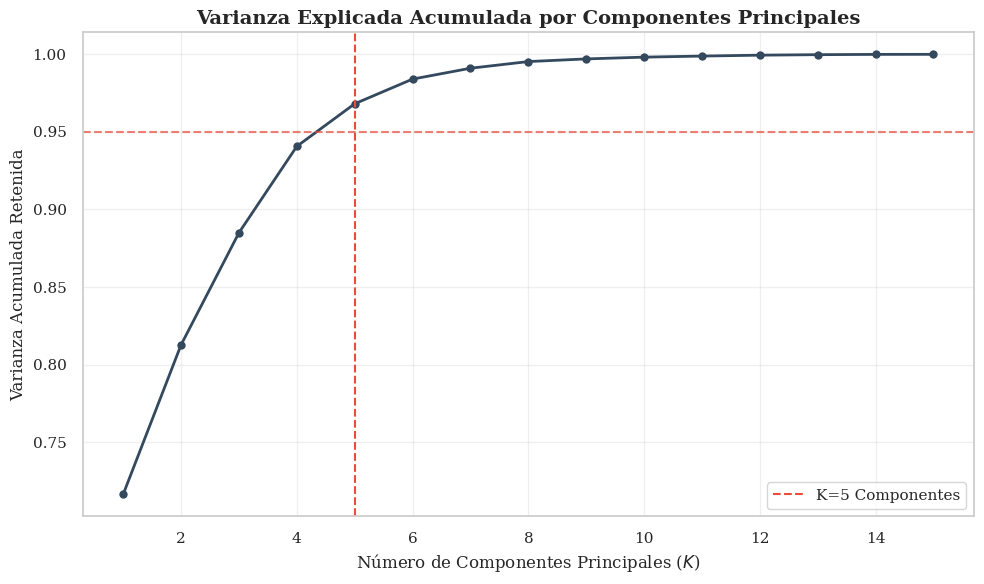
\includegraphics[width=0.90\textwidth]{img/cell13_out1.png}
\caption{Varianza acumulada explicada por componente principal, con el punto de corte $K=5$ para retener el 95\% de la varianza.}
\label{fig:pca}
\end{figure}
 
Se descartaron técnicas de reducción no lineal como \emph{t-SNE}, dado que el objetivo era preservar un mapeo afín de las varianzas continuas útil para un clasificador de particiones ortogonales, propiedad que la no linealidad estocástica no garantiza.
\section{Metodología Propuesta}\label{sec:methodology}
 
\subsection{Pipeline general}
El pipeline metodológico propuesto se estructura en las siguientes etapas secuenciales: (1) ingesta y diagnóstico de anomalías; (2) corrección de códigos de error de sensor; (3) ingeniería de la variable objetivo con prevención de \emph{data leakage}; (4) partición estratificada; (5) imputación por mediana y escalamiento robusto ajustados únicamente sobre el conjunto de entrenamiento; (6) reducción de dimensionalidad mediante PCA; (7) entrenamiento y optimización de un Random Forest Classifier balanceado; (8) evaluación integral sobre el conjunto de prueba. La Fig. \ref{fig:pipeline} resume esta arquitectura.
 
\begin{figure}[H]
\centering
\begin{verbatim}
%% DIAGRAMA MERMAID (a convertir a figura IEEE)
%% graph TD
%%   A[Ingesta DATASET.csv] --> B[Diagnostico EDA -999]
%%   B --> C[Correccion NaN]
%%   C --> D[Target_Helada + eliminacion leakage]
%%   D --> E[Split 80/20 estratificado]
%%   E --> F[Imputacion mediana + RobustScaler]
%%   F --> G[PCA K=5, 95% varianza]
%%   G --> H[RandomForest + GridSearchCV]
%%   H --> I[Evaluacion: ROC, PR, Kappa]
\end{verbatim}
\caption{Diagrama de flujo del pipeline metodológico propuesto (representación textual Mermaid, pendiente de conversión a figura vectorial IEEE).}
\label{fig:pipeline}
\end{figure}
 
\subsection{Algoritmo de clasificación}
Se seleccionó un ensamble de árboles de decisión (\emph{Random Forest Classifier}) por su afinidad geométrica con particiones ortogonales del espacio, coherente con la naturaleza del subespacio generado por PCA. El modelo se configuró con ponderación balanceada de clases (\texttt{class\_weight='balanced'}) para compensar el desbalance de clases documentado en la Sección III-G, ajustando los pesos de manera inversamente proporcional a la frecuencia de cada clase:
\begin{equation}
w_c = \frac{N}{2 \cdot N_c}
\label{eq:classweight}
\end{equation}
donde $N$ es el número total de instancias y $N_c$ el número de instancias de la clase $c$.
 
\subsection{Función objetivo y optimización de hiperparámetros}
La optimización se realizó mediante \texttt{GridSearchCV} con validación cruzada de 3 particiones (\emph{3-fold}), utilizando como función objetivo el F1-Score Macro:
\begin{equation}
F1_{macro} = \frac{1}{C} \sum_{c=1}^{C} \frac{2 \cdot P_c \cdot R_c}{P_c + R_c}
\label{eq:f1macro}
\end{equation}
donde $P_c$ y $R_c$ son la precisión y el \emph{recall} de la clase $c$, respectivamente. Esta métrica fue elegida en lugar de la exactitud (\emph{accuracy}), ya que, dado el desbalance del 83.76\% frente a 16.24\%, un clasificador trivial que prediga siempre la clase mayoritaria superaría el 90\% de exactitud sin ninguna utilidad práctica.
 
La Tabla \ref{tab:grid} resume el espacio de búsqueda de hiperparámetros explorado.
 
\begin{table}[H]
\centering
\caption{Espacio de búsqueda de hiperparámetros (\texttt{GridSearchCV})}
\label{tab:grid}
\begin{tabular}{lll}
\toprule
\textbf{Hiperparámetro} & \textbf{Valores explorados} & \textbf{Descripción} \\
\midrule
\texttt{n\_estimators} & \{50, 100\} & Número de árboles \\
\texttt{max\_depth} & \{5, 10\} & Profundidad máxima \\
\texttt{min\_samples\_split} & \{2, 5\} & Mínimo de muestras por nodo \\
\bottomrule
\end{tabular}
\end{table}
 
La grilla resultante comprende 8 combinaciones de hiperparámetros, evaluadas mediante validación cruzada de 3 particiones, totalizando 24 ajustes de modelo. Se utilizó \texttt{n\_jobs=-1} para paralelizar el cómputo sobre todos los núcleos disponibles del entorno de ejecución.
 
\subsection{Validación}
Los hiperparámetros óptimos obtenidos fueron $\texttt{max\_depth}=10$, $\texttt{min\_samples\_split}=2$ y $\texttt{n\_estimators}=100$, alcanzando un F1-Score Macro interno de validación cruzada de $0.8330$.
\section{Implementación del Software}\label{sec:implementation}

\subsection{Entorno tecnológico}
El desarrollo se realizó íntegramente en \emph{Google Colab}, sobre un cuaderno
Jupyter (formato \texttt{.ipynb}) ejecutado con un kernel de Python~3. El
paradigma de cómputo es exclusivamente \emph{CPU}; no se emplearon librerías de
aprendizaje profundo (PyTorch, TensorFlow) ni implementaciones de \emph{gradient
boosting} (XGBoost, LightGBM), dado que el clasificador seleccionado ---un
ensamble Random Forest--- está disponible de forma nativa en \emph{scikit-learn}.
Cabe señalar, como contraste, que el autor original del repositorio de datos
empleó un clasificador XGBoost sobre la versión filtrada del conjunto; el presente
trabajo constituye un pipeline independiente basado en scikit-learn.

La Tabla~\ref{tab:stack} resume el ecosistema de librerías identificado en las
celdas de importación del cuaderno.

\begin{table}[H]
\centering
\caption{Ecosistema tecnológico del proyecto}
\label{tab:stack}
\footnotesize
\renewcommand{\arraystretch}{1.2}
\begin{tabular}{p{2.2cm}p{5.4cm}}
\toprule
\textbf{Librería} & \textbf{Rol en el pipeline} \\
\midrule
\texttt{numpy} & Álgebra vectorial y control de semilla aleatoria \\
\texttt{pandas} & Estructura de datos tabular e ingesta \\
\texttt{matplotlib} & Visualización científica base \\
\texttt{seaborn} & Visualización estadística (densidades, heatmaps) \\
\texttt{kagglehub} & Ingesta programática del dataset desde Kaggle \\
\texttt{scikit-learn} & Preprocesamiento, PCA, modelado, evaluación \\
\bottomrule
\end{tabular}
\end{table}

Dentro de \emph{scikit-learn}, los módulos utilizados son:
\texttt{model\_selection} (\texttt{train\_test\_split}, \texttt{GridSearchCV}),
\texttt{pipeline} (\texttt{Pipeline}), \texttt{impute} (\texttt{SimpleImputer}),
\texttt{preprocessing} (\texttt{RobustScaler}), \texttt{compose}
(\texttt{ColumnTransformer}), \texttt{decomposition} (\texttt{PCA}),
\texttt{ensemble} (\texttt{RandomForestClassifier}) y \texttt{metrics}
(\texttt{classification\_report}, \texttt{confusion\_matrix},
\texttt{roc\_curve}, \texttt{auc}, \texttt{precision\_recall\_curve},
\texttt{average\_precision\_score}, \texttt{cohen\_kappa\_score},
\texttt{make\_scorer}, \texttt{f1\_score}).

\subsection{Organización modular del código}
El proyecto se implementó como un cuaderno lineal estructurado en bloques
funcionales cohesivos, en lugar de un paquete distribuido en un directorio
\texttt{/src}. Cada bloque encapsula una etapa del pipeline y expone sus
resultados a la siguiente mediante variables de estado explícitas. La
Tabla~\ref{tab:modules} describe esta organización modular por bloques.

\begin{table}[H]
\centering
\caption{Organización modular del cuaderno por bloques funcionales}
\label{tab:modules}
\footnotesize
\renewcommand{\arraystretch}{1.2}
\begin{tabular}{p{1.0cm}p{3.0cm}p{3.4cm}}
\toprule
\textbf{Bloque} & \textbf{Responsabilidad} & \textbf{Artefactos producidos} \\
\midrule
1 & Configuración global e ingesta & \texttt{df}, semilla global \\
2 & Diagnóstico y corrección de anomalías & \texttt{df} corregido, tasa de nulos \\
3 & Ingeniería de etiqueta y correlación & \texttt{Target\_Helada}, matriz Pearson \\
4 & Partición y preprocesamiento & \texttt{Pipeline}, \texttt{X\_train/test} escalados \\
5 & Reducción de dimensionalidad & \texttt{PCA}, \texttt{X\_train/test\_pca} \\
6 & Modelado y optimización & \texttt{best\_model}, hiperparámetros \\
7 & Evaluación integral & métricas, curvas ROC/PR, Kappa \\
\bottomrule
\end{tabular}
\end{table}

El preprocesamiento se encapsuló mediante los abstractores composicionales de
scikit-learn: un \texttt{Pipeline} que encadena \texttt{SimpleImputer} y
\texttt{RobustScaler}, integrado a su vez en un \texttt{ColumnTransformer}. Este
diseño garantiza que las transformaciones se ajusten (\emph{fit}) exclusivamente
sobre el conjunto de entrenamiento y se apliquen (\emph{transform}) de forma ciega
sobre el conjunto de prueba, previniendo la fuga de información estadística entre
particiones.

\subsection{Gestión de dependencias}
Las dependencias se gestionan a través del entorno preinstalado de Google Colab,
complementado por una instrucción de instalación explícita
(\texttt{pip install kagglehub[pandas-datasets] seaborn matplotlib scikit-learn})
documentada en la primera celda del cuaderno. El proyecto no fija versiones
específicas mediante un archivo \texttt{requirements.txt} o \texttt{environment.yml};
la adopción de un manifiesto de dependencias con versiones ancladas se plantea
como una mejora para robustecer la reproducibilidad a largo plazo.

\subsection{Reproducibilidad determinista}
El determinismo del pipeline se garantiza mediante la fijación de una semilla
global $\text{SEED}=42$, propagada por una función dedicada,
\texttt{set\_global\_seed}, que controla las tres fuentes de aleatoriedad activas
en el entorno de ejecución:
\begin{enumerate}
\item \texttt{random.seed(seed)} --- generador pseudoaleatorio de la biblioteca
estándar de Python.
\item \texttt{np.random.seed(seed)} --- generador de NumPy, base de las
operaciones estocásticas de scikit-learn.
\item \texttt{os.environ['PYTHONHASHSEED'] = str(seed)} --- fijación del hash de
Python para estabilizar el orden de estructuras dependientes de hashing.
\end{enumerate}

Esta misma semilla se reutiliza de forma consistente en cada componente
estocástico del pipeline: el muestreo de la matriz de correlación
(\texttt{sample(random\_state=SEED)}), la partición estratificada
(\texttt{train\_test\_split(random\_state=SEED)}), la descomposición espectral
(\texttt{PCA(random\_state=SEED)}) y la inicialización del ensamble
(\texttt{RandomForestClassifier(random\_state=SEED)}). Dado que el cómputo se
ejecuta enteramente sobre CPU mediante scikit-learn, no intervienen fuentes de no
determinismo asociadas a aceleradores por hardware (p.\,ej. operaciones no
deterministas de CUDA/cuDNN), por lo que no se requieren mecanismos adicionales de
control de aleatoriedad a nivel de GPU. La reproducibilidad experimental queda así
garantizada de extremo a extremo bajo el entorno descrito.
\section{Resultados Experimentales y Análisis Estadístico}\label{sec:results}

\subsection{Métricas de clasificación sobre el conjunto de prueba}
El modelo campeón se evaluó sobre el conjunto de prueba
($N_{test}=334\,566$), que permaneció aislado durante todo el proceso de
optimización. La Tabla~\ref{tab:classreport} presenta el reporte de clasificación
completo, generado con cuatro decimales de precisión.

\begin{table}[H]
\centering
\caption{Reporte de clasificación sobre el conjunto de prueba}
\label{tab:classreport}
\footnotesize
\begin{tabular}{lcccc}
\toprule
\textbf{Clase} & \textbf{Precision} & \textbf{Recall} & \textbf{F1-Score} & \textbf{Soporte} \\
\midrule
0 (Normal) & 0.9835 & 0.8859 & 0.9322 & 280\,224 \\
1 (Helada) & 0.6109 & 0.9234 & 0.7353 & 54\,342 \\
\midrule
\textit{Accuracy} & \multicolumn{3}{c}{0.8920} & 334\,566 \\
\textit{Macro avg} & 0.7972 & 0.9047 & 0.8338 & 334\,566 \\
\textit{Weighted avg} & 0.9230 & 0.8920 & 0.9002 & 334\,566 \\
\bottomrule
\end{tabular}
\end{table}

El modelo alcanzó un \emph{Recall} de $92.34\%$ para la clase minoritaria
(helada), a costa de una \emph{Precision} de $61.09\%$ en dicha clase. Este
compromiso es deliberado y coherente con el objetivo operativo de minimizar los
falsos negativos en un contexto de prevención de desastres agrometeorológicos:
en un sistema de alerta temprana, omitir una helada real (falso negativo) tiene un
costo agrícola muy superior al de emitir una alerta que no se materializa (falso
positivo).

\subsection{Métricas globales robustas al desbalance}
Dado el desbalance de clases documentado en la Sección~\ref{sec:dataset}, se
reportan métricas específicamente robustas frente a distribuciones asimétricas.
La Tabla~\ref{tab:globalmetrics} consolida las métricas globales del modelo.

\begin{table}[H]
\centering
\caption{Métricas globales del modelo campeón}
\label{tab:globalmetrics}
\footnotesize
\renewcommand{\arraystretch}{1.2}
\begin{tabular}{lc}
\toprule
\textbf{Métrica} & \textbf{Valor} \\
\midrule
Exactitud (\emph{Accuracy}) & 0.8920 \\
F1-Score Macro (validación interna, 3-fold) & 0.8330 \\
F1-Score Macro (conjunto de prueba) & 0.8338 \\
Índice Kappa de Cohen ($\kappa$) & 0.6710 \\
Área bajo la curva ROC (ROC-AUC) & 0.9690 \\
\bottomrule
\end{tabular}
\end{table}

El índice Kappa de Cohen de $\kappa=0.6710$ indica una concordancia
\emph{sustancial} entre las predicciones y las etiquetas reales, según la escala
de interpretación convencional, descontando los aciertos atribuibles al azar. El
área bajo la curva ROC de $0.9690$ evidencia una elevada capacidad discriminante
global del clasificador. La estrecha correspondencia entre el F1-Score Macro de
validación interna ($0.8330$) y el de prueba ($0.8338$) sugiere ausencia de
sobreajuste significativo y buena capacidad de generalización.

\subsection{Matriz de confusión y curvas de desempeño}
La Fig.~\ref{fig:eval} presenta, de izquierda a derecha, la matriz de confusión,
la curva ROC y la curva Precision-Recall obtenidas sobre el conjunto de prueba.
La curva Precision-Recall es particularmente informativa en escenarios
desbalanceados, ya que evalúa directamente la capacidad de aislar la clase
minoritaria sin verse favorecida por el gran volumen de verdaderos negativos.

\begin{figure*}[t]
\centering
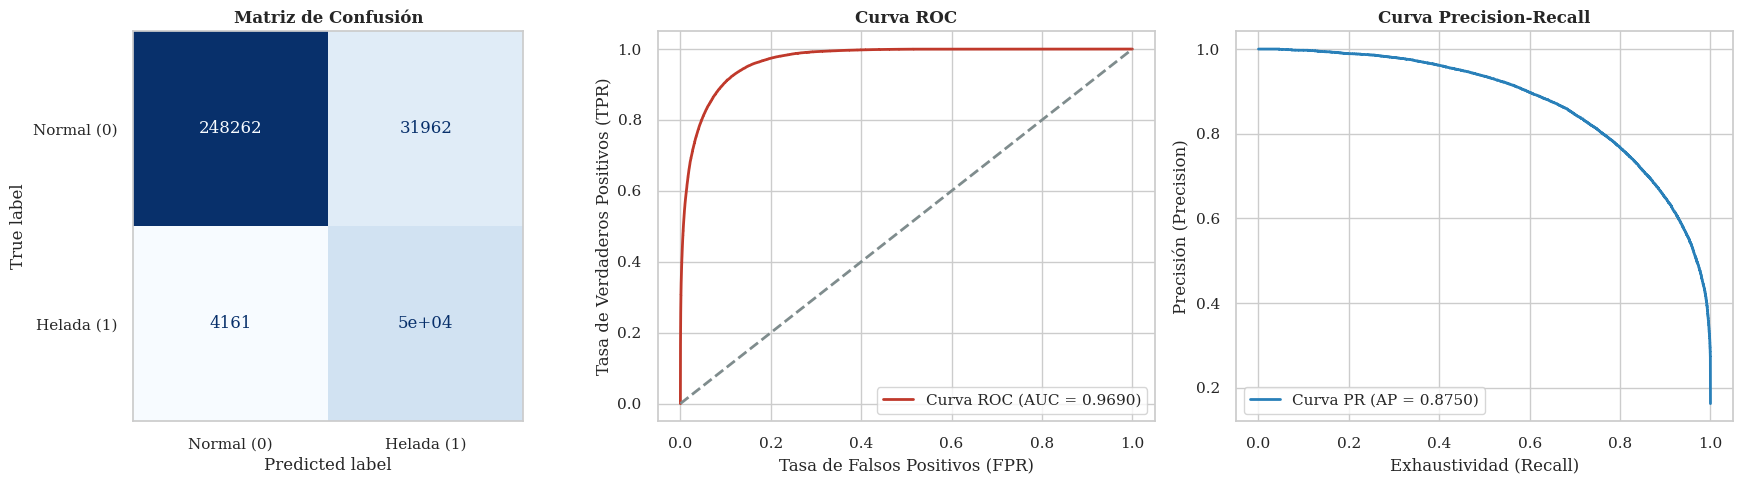
\includegraphics[width=0.95\textwidth]{img/cell19_out1.png}
\caption{Evaluación integral del modelo campeón sobre el conjunto de prueba:
matriz de confusión (izquierda), curva ROC con AUC$=0.9690$ (centro) y curva
Precision-Recall (derecha).}
\label{fig:eval}
\end{figure*}

\subsection{Importancia de los componentes principales}
La Fig.~\ref{fig:importance} presenta la reducción media de impureza de Gini
atribuida a cada componente principal por el ensamble. El hallazgo más relevante
es que la capacidad discriminante del modelo no reside en la dirección de mayor
varianza global (PC1), sino en componentes latentes ortogonales específicos,
identificados como PC3 y PC2. Esto revela que la señal predictiva de la helada
habita en direcciones de varianza intermedia y no en la dominante, un resultado
no trivial desde la perspectiva del análisis espectral.

\begin{figure}[H]
\centering
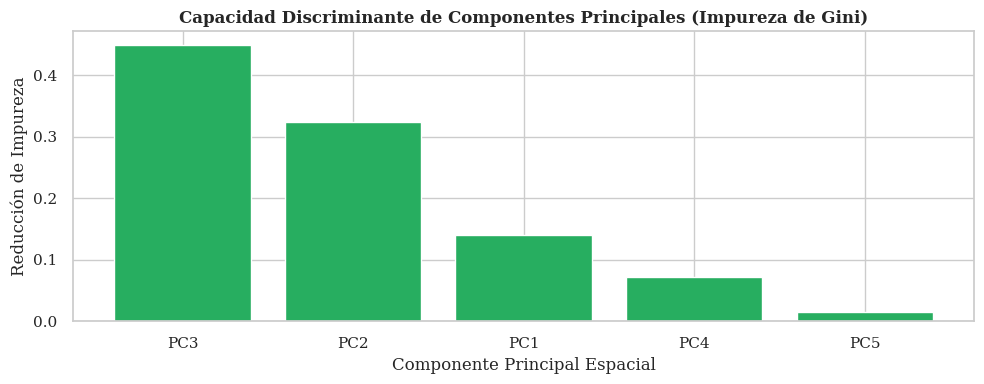
\includegraphics[width=0.90\textwidth]{img/cell19_out2.png}
\caption{Capacidad discriminante (impureza de Gini) de los componentes
principales empleados por el modelo campeón.}
\label{fig:importance}
\end{figure}

\subsection{Análisis estadístico de significancia}
El diseño experimental documentado no permite realizar un análisis estadístico
inferencial de significancia. La aplicación de pruebas como la de Wilcoxon
(comparación pareada de dos modelos), ANOVA (comparación de tres o más modelos) o
el procedimiento post-hoc de Tukey requiere dos condiciones que el pipeline actual
no satisface: (i) la existencia de \emph{múltiples modelos de línea base}
entrenados bajo protocolo idéntico para su contraste, y (ii) la disponibilidad de
\emph{múltiples ejecuciones independientes} por modelo (p.\,ej. mediante semillas
distintas o validación cruzada repetida) que provean las distribuciones de
métricas sobre las cuales aplicar dichas pruebas.

En su estado actual, el experimento entrena un único modelo (Random Forest
optimizado) con una semilla fija ($\text{SEED}=42$) y lo evalúa una sola vez sobre
un único conjunto de prueba. En consecuencia:

\begin{quote}
\emph{El análisis estadístico inferencial no pudo realizarse debido a que el
notebook no conserva múltiples ejecuciones independientes necesarias para aplicar
pruebas de significancia.}
\end{quote}

Para habilitar este análisis en trabajos futuros, se propone el siguiente
protocolo experimental: (1) entrenar un conjunto de modelos de línea base
(p.\,ej. Regresión Logística, SVM, XGBoost) bajo el mismo pipeline de
preprocesamiento; (2) ejecutar validación cruzada estratificada de $k$ particiones
repetida $r$ veces con semillas distintas, registrando el F1-Score Macro de cada
repetición; (3) aplicar la prueba de Friedman para detectar diferencias globales
entre modelos y, de resultar significativa, el post-hoc de Nemenyi (o Wilcoxon con
corrección de Bonferroni para comparaciones pareadas contra el modelo propuesto).
Este diseño proporcionaría la evidencia estadística necesaria para afirmar que las
diferencias de rendimiento no son producto del azar experimental.
\section{Discusión de Resultados}\label{sec:discussion}

\subsection{Idoneidad del algoritmo frente a las propiedades de los datos}
La elección de un ensamble Random Forest no fue arbitraria, sino una consecuencia
directa de las propiedades intrínsecas del conjunto de datos reveladas durante el
análisis exploratorio. Cuatro características del dominio favorecieron
específicamente a este algoritmo frente a alternativas.

Primero, el EDA evidenció \emph{alta multicolinealidad} entre grupos de sensores
relacionados (variantes de viento y de temperatura). Los árboles de decisión que
componen el bosque realizan particiones ortogonales del espacio de
características, lo que los hace intrínsecamente robustos a la redundancia lineal
entre predictores; combinados con la reducción de dimensionalidad vía PCA, que
descorrelaciona explícitamente el espacio, se obtuvo una sinergia geométrica
favorable a las particiones axiales del ensamble. Un modelo lineal como la
regresión logística habría sufrido de inestabilidad en sus coeficientes ante esta
multicolinealidad.

Segundo, el conjunto presentaba \emph{ruido de instrumentación} en forma del
código \texttt{-999} y \emph{outliers univariados legítimos} (precipitación de
hasta $470$\,mm). Random Forest es notablemente tolerante a valores atípicos, dado
que sus divisiones se basan en umbrales ordinales y no en distancias métricas
absolutas; esto contrasta con algoritmos sensibles a la escala como SVM con
kernel RBF o $k$-NN, cuyo desempeño se habría degradado sin un tratamiento de
outliers más agresivo. La combinación con \texttt{RobustScaler} reforzó esta
tolerancia al centrar y escalar mediante estadísticos resistentes (mediana e
IQR).

Tercero, el problema exhibió un \emph{desbalance de clases severo} ($16.24\%$
frente a $83.76\%$). La capacidad de Random Forest de incorporar ponderación de
clases (\texttt{class\_weight='balanced'}) permitió reajustar la función de
decisión hacia la clase minoritaria sin recurrir a generación sintética de
muestras, cuyo uso ---según se discutió en el estado del arte--- puede magnificar
la complejidad de datos ya ruidosos. La optimización sobre F1-Score Macro alineó
directamente la función objetivo con la métrica operativamente relevante.

Cuarto, la señal predictiva resultó \emph{no trivial en su ubicación espectral}:
el análisis de impureza de Gini reveló que la capacidad discriminante reside en
componentes de varianza intermedia (PC3, PC2) y no en la dirección dominante
(PC1). La naturaleza no paramétrica de Random Forest, capaz de capturar
interacciones no lineales entre componentes sin asumir una forma funcional
predeterminada, resultó adecuada para explotar una señal distribuida de esta
manera, algo que un clasificador lineal sobre PC1 no habría capturado.

\subsection{Interpretación del compromiso Precision--Recall}
El resultado central ---un \emph{Recall} de $92.34\%$ frente a una \emph{Precision}
de $61.09\%$ en la clase de helada--- debe interpretarse a la luz del contexto de
aplicación y no como una deficiencia. En un sistema de alerta temprana
agrometeorológica, la matriz de costos es marcadamente asimétrica: el costo de un
falso negativo (una helada no anticipada que destruye un cultivo) supera
ampliamente el de un falso positivo (una alerta preventiva que no se materializa).
La ponderación de clases y la optimización sobre F1-Macro desplazaron
deliberadamente el modelo hacia la sensibilidad, priorizando la detección
exhaustiva de eventos críticos. El elevado ROC-AUC ($0.9690$) confirma que esta
sensibilidad no se obtuvo a costa de una capacidad discriminante global pobre.

\subsection{Amenazas a la validez interna}
La validez interna se refiere a si las conclusiones del experimento son correctas
dentro del entorno controlado del estudio. Se identifican las siguientes
amenazas.

\emph{Prevención de fuga de información.} El riesgo más severo ---la fuga por
predicción tautológica--- fue mitigado explícitamente al eliminar
\texttt{temp\_min\_2m} del espacio de predictores tras derivar de ella la etiqueta.
Asimismo, todos los parámetros de imputación y escalamiento se ajustaron
exclusivamente sobre el conjunto de entrenamiento, transformando el de prueba de
forma ciega. No obstante, el ajuste de PCA también se realizó sobre el conjunto
de entrenamiento, lo cual es metodológicamente correcto, pero su interacción con
la ponderación de clases no fue objeto de una validación anidada, lo que
constituye una amenaza residual menor.

\emph{Sesgo de selección en la matriz de correlación.} El análisis de correlación
de Pearson se computó sobre una submuestra de $20\,000$ registros completos, no
sobre la totalidad del conjunto. Aunque la submuestra fue aleatoria y con semilla
fija, la exclusión de registros con nulos (\texttt{dropna}) podría introducir un
sesgo si la ausencia de datos no fuese completamente aleatoria (MCAR). Dado que
los faltantes provienen de fallos de sensor uniformemente distribuidos
($0.03\%$), este sesgo se considera despreciable, pero no puede descartarse
formalmente.

\emph{Ausencia de validación estadística.} Como se detalló en la
Sección~\ref{sec:results}, el experimento no incluye múltiples ejecuciones
independientes ni modelos de línea base, por lo que no es posible afirmar con
respaldo estadístico que el desempeño observado sea significativamente superior al
de alternativas. Las conclusiones se sustentan en un único punto experimental, lo
que constituye la principal amenaza a la validez interna del estudio.

\subsection{Amenazas a la validez externa}
La validez externa concierne a la capacidad de generalización del modelo a
entornos productivos fuera del conjunto de prueba.

\emph{Representatividad geográfica y temporal.} El conjunto abarca estaciones
peruanas en un rango de latitud $[-18.01, -8.19]$ y altitud
$[1079, 4691]$\,m.s.n.m., a lo largo del periodo 2000--2025. La generalización a
microclimas no representados en esta cobertura, o a regiones de menor altitud, no
está garantizada. La helada es un fenómeno intrínsecamente local, y un modelo
entrenado sobre estas estaciones podría degradar su desempeño en ubicaciones con
regímenes térmicos distintos.

\emph{Deriva de distribución (\emph{dataset shift}).} En un despliegue productivo,
los patrones climáticos pueden desviarse de la distribución de entrenamiento por
efecto de la variabilidad climática de largo plazo. Un modelo estático como el
presentado requeriría reentrenamiento periódico para mantener su validez ante
posibles cambios en las distribuciones marginales de las variables.

\emph{Dependencia de la calidad de instrumentación.} El pipeline asume que los
fallos de sensor se codifican mediante el valor \texttt{-999}. En un entorno
productivo con sensores heterogéneos que empleen otros códigos de error o que
produzcan lecturas corruptas de forma no señalizada, el mecanismo de corrección
podría no capturar todas las anomalías, comprometiendo la robustez del sistema.

\emph{Ausencia de estructura temporal explícita.} El modelo trata cada
observación de forma independiente, sin incorporar descriptores espaciotemporales
(estacionalidad, tendencia). En producción, la predicción anticipada de heladas
se beneficiaría de una formulación que capture la dinámica temporal, lo que
sugiere que el desempeño en un escenario de pronóstico real (a $t+k$ horas) podría
diferir del obtenido en la clasificación sobre observaciones concurrentes.
\section{Conclusiones y Trabajo Futuro}\label{sec:conclusions}

\subsection{Conclusiones técnicas}
Este trabajo desarrolló y evaluó un pipeline reproducible de minería de datos
para la predicción binaria de heladas en el territorio peruano, sobre un conjunto
de $1\,672\,827$ observaciones meteorológicas. De la evidencia experimental se
extraen las siguientes conclusiones directas:

\begin{enumerate}
\item El ensamble Random Forest optimizado alcanzó un \emph{Recall} de $92.34\%$
en la detección de heladas y un ROC-AUC de $0.9690$, con un índice Kappa de Cohen
de $0.6710$ (concordancia sustancial), validando el sistema como una herramienta
de alerta temprana de alta sensibilidad.
\item La estrategia de ponderación balanceada de clases combinada con
optimización directa sobre F1-Score Macro resultó eficaz para manejar un
desbalance severo ($16.24\%$ frente a $83.76\%$) sin recurrir a generación
sintética de muestras, evitando así la amplificación de la complejidad de datos
ya afectados por ruido de instrumentación.
\item La cercanía entre el F1-Score Macro de validación interna ($0.8330$) y el de
prueba ($0.8338$) evidencia una capacidad de generalización estable y ausencia de
sobreajuste significativo dentro del dominio del conjunto evaluado.
\item El pipeline de escalamiento robusto (\texttt{RobustScaler}) seguido de PCA
redujo la dimensionalidad de 15 a 5 componentes reteniendo el $95\%$ de la
varianza, demostrando que el problema admite una representación compacta sin
pérdida sustancial de capacidad predictiva.
\end{enumerate}

\subsection{Lecciones aprendidas sobre los datos y la ingeniería de características}
El proceso de desarrollo dejó tres aprendizajes de valor sobre el comportamiento
de los datos y su preparación.

Primero, el diagnóstico visual exploratorio previo a cualquier transformación
matemática resultó indispensable: el código de error de sensor \texttt{-999} se
encontraba enmascarado y no habría sido detectado por una inspección estructural
convencional (\texttt{df.info()} reportaba cero nulos). Su omisión habría
distorsionado irreversiblemente tanto la matriz de correlación como el
escalamiento, comprometiendo todo el análisis posterior. Esto confirma que un
conjunto declarado ``preprocesado'' por su fuente exige, no obstante, una
auditoría de calidad independiente.

Segundo, la ingeniería de la variable objetivo demostró que la prevención de fuga
de información es un requisito de diseño y no un detalle: conservar
\texttt{temp\_min\_2m} entre los predictores habría inducido una regla
determinista trivial con una correlación artificial cercana a $-1$, ocultando las
verdaderas relaciones climáticas del sistema.

Tercero, el análisis de impureza de Gini reveló que la capacidad discriminante no
reside en la dirección de mayor varianza global (PC1), sino en componentes
latentes de varianza intermedia (PC3, PC2). Esta lección advierte contra la
suposición ingenua de que las primeras componentes principales concentran
siempre la señal predictiva más relevante.

\subsection{Trabajo futuro}
Se identifican cuatro líneas de trabajo futuro de carácter metodológico.

\emph{Validación estadística rigurosa.} La línea prioritaria consiste en dotar al
estudio de respaldo inferencial mediante la incorporación de modelos de línea base
(Regresión Logística, SVM, XGBoost) entrenados bajo el mismo pipeline, ejecutando
validación cruzada estratificada repetida con múltiples semillas y aplicando
pruebas de significancia (Friedman con post-hoc de Nemenyi, o Wilcoxon con
corrección de Bonferroni) para contrastar formalmente el modelo propuesto frente a
las alternativas.

\emph{Enriquecimiento de características espaciotemporales.} Se propone incorporar
descriptores que capturen la dinámica temporal del fenómeno, en particular una
codificación trigonométrica (seno/coseno) de las variables cíclicas de día y mes,
así como reformular el problema como un pronóstico a $t+k$ horas en lugar de una
clasificación sobre observaciones concurrentes, acercando el sistema a un
escenario operativo real de alerta anticipada.

\emph{Exploración de arquitecturas profundas.} Dada la escala del conjunto (más de
1.6 millones de observaciones), resulta pertinente evaluar arquitecturas de
aprendizaje profundo ---redes recurrentes (LSTM/GRU) o convolucionales
temporales--- capaces de modelar dependencias secuenciales, contrastándolas con el
ensamble Random Forest como línea base robusta.

\emph{Técnicas de rebalanceo y aprendizaje semisupervisado.} Se plantea explorar
técnicas de generación sintética adaptativa (ADASYN) sobre el espacio de
entrenamiento para intentar reducir la tasa de falsos positivos sin sacrificar la
sensibilidad alcanzada, así como estrategias de aprendizaje semisupervisado que
aprovechen registros meteorológicos no etiquetados de estaciones adicionales para
mejorar la generalización geográfica del modelo.
% --- SECCIÓN DE REFERENCIAS ---
\renewcommand{\refname}{Referencias Bibliográficas}
\begin{thebibliography}{99}

\bibitem{diedrichs2018}
A. L. Diedrichs, F. Bromberg, D. Dujovne, K. Brun-Laguna, and T. Watteyne,
``Prediction of Frost Events Using Machine Learning and IoT Sensing Devices,''
\emph{IEEE Internet of Things Journal}, vol. 5, no. 6, pp. 4589--4597, Dec. 2018.

\bibitem{talsma2023}
C. J. Talsma, K. C. Solander, M. K. Mudunuru, B. Crawford, and M. R. Powell,
``Frost prediction using machine learning and deep neural network models,''
\emph{Frontiers in Artificial Intelligence}, vol. 5, art. no. 963781, 2023,
doi: 10.3389/frai.2022.963781.

\bibitem{rozante2023}
J. R. Rozante, E. Ramirez, D. Ramirez, and G. Rozante,
``Improved frost forecast using machine learning methods,''
\emph{Artificial Intelligence in Agriculture}, 2023.

\bibitem{perez2025}
J. Pérez Tárraga, M. Castillo-Cara, E. Arias-Antúnez, and D. Dujovne,
``Frost forecasting through machine learning algorithms,''
\emph{Earth Science Informatics}, vol. 18, no. 2, art. no. 183, 2025,
doi: 10.1007/s12145-025-01710-6.

\bibitem{azhar2023}
N. A. Azhar, M. S. Mohd Pozi, A. Mohamed Din, and A. Jatowt,
``An Investigation of SMOTE Based Methods for Imbalanced Datasets With Data
Complexity Analysis,'' \emph{IEEE Transactions on Knowledge and Data
Engineering}, vol. 35, no. 7, pp. 6651--6672, Jul. 2023,
doi: 10.1109/TKDE.2022.3179381.

\bibitem{wang2021}
L. Wang, M. Han, X. Li, N. Zhang, and H. Cheng,
``Review of Classification Methods on Unbalanced Data Sets,''
\emph{IEEE Access}, vol. 9, pp. 64606--64628, 2021,
doi: 10.1109/ACCESS.2021.3074243.

\bibitem{chawla2002}
N. V. Chawla, K. W. Bowyer, L. O. Hall, and W. P. Kegelmeyer,
``SMOTE: Synthetic Minority Over-sampling Technique,''
\emph{Journal of Artificial Intelligence Research}, vol. 16, pp. 321--357, 2002.

\bibitem{zhao2024}
M. Zhao,
``Synthetic minority oversampling technique based on natural neighborhood graph
with subgraph cores for class-imbalanced classification,''
\emph{The Journal of Supercomputing}, vol. 81, 2024,
doi: 10.1007/s11227-024-06655-z.

\bibitem{swana2022}
E. F. Swana, W. Doorsamy, and P. Bokoro,
``Tomek Link and SMOTE Approaches for Machine Fault Classification With an
Imbalanced Dataset,'' \emph{Sensors}, vol. 22, no. 9, art. no. 3246, 2022.

\bibitem{imani2025}
M. Imani, A. Beikmohammadi, and H. R. Arabnia,
``Comprehensive Analysis of Random Forest and XGBoost Performance with SMOTE,
ADASYN, and GNUS Under Varying Imbalance Levels,''
\emph{Technologies}, vol. 13, no. 3, art. no. 88, 2025.

\bibitem{galvan2022}
I. M. Galván \emph{et al.},
``A combination of supervised dimensionality reduction and learning methods to
forecast solar radiation,'' \emph{Applied Intelligence}, 2022,
doi: 10.1007/s10489-022-04175-y.

\bibitem{bujang2021}
S. D. A. Bujang \emph{et al.},
``Multiclass Prediction Model for Student Grade Prediction Using Machine
Learning,'' \emph{IEEE Access}, vol. 9, pp. 95608--95621, 2021,
doi: 10.1109/ACCESS.2021.3093563.

\bibitem{chen2024soil}
P.-Y. Chen, C.-C. Chen, C. Kang, J.-W. Liu, and Y.-H. Li,
``Soil water content prediction across seasons using random forest based on
precipitation-related data,'' \emph{Computers and Electronics in Agriculture},
vol. 230, art. no. 109802, 2025.

\bibitem{breiman2001}
L. Breiman, ``Random Forests,'' \emph{Machine Learning}, vol. 45, no. 1,
pp. 5--32, 2001.

\bibitem{pedregosa2011}
F. Pedregosa \emph{et al.}, ``Scikit-learn: Machine Learning in Python,''
\emph{Journal of Machine Learning Research}, vol. 12, pp. 2825--2830, 2011.

\end{thebibliography}

\end{document}